\chapter{Orbital Atom: Bentuk, Energi, dan Ukuran}\label{ch:b2:atomic-orbitals}

Atom hidrogen tidak mempunyai tepi: elektronnya dapat ditemukan pada jarak
berapa pun dari inti, dengan peluang yang cepat menurun tetapi tidak
pernah mencapai nol. Namun atom mempunyai ukuran, dan atom natrium sekitar
dua kali lebih lebar daripada atom klor, walaupun mengandung lebih sedikit
elektron. Jilid Tahun 1 menamai keadaan-keadaan elektron dengan tiga
bilangan kuantum; di sini setiap keadaan menjadi fungsi posisi, dengan
bentuk, simpul, tanda, dan ukuran, dan seperangkat aturan sederhana
mengubahnya menjadi \omterm{def:b2:atomic-orbitals:orbital-energy}{energi orbital} untuk atom apa pun. Bentuk dan tanda
inilah yang digabungkan oleh empat bab berikutnya menjadi orbital molekul.

\begin{recall}
Jilid Tahun 1: bilangan kuantum $n$, $l$, $m_l$, $m_s$; orbital atom sebagai
keadaan $(n, l, m_l)$; kulit dan subkulit; penapisan dan muatan inti efektif
(secara kualitatif); konfigurasi elektron; tingkat-tingkat energi hidrogen,
$-E_R/n^2$ dengan $E_R = \qty{13.6}{eV}$. Dari fisika: \omterm{def:b2:atomic-orbitals:wavefunction}{fungsi gelombang},
yang kuadrat modulusnya merupakan \omterm{def:b2:atomic-orbitals:wavefunction}{kepadatan peluang}.
\end{recall}

\section{Fungsi gelombang atom hidrogen}

\begin{definition}[Fungsi gelombang]\label{def:b2:atomic-orbitals:wavefunction}
Keadaan sebuah elektron diperikan oleh \emph{fungsi gelombang}\index{fungsi gelombang}
$\psi(x, y, z)$; $|\psi|^2$ adalah \emph{kepadatan peluangnya}
\index{kepadatan peluang}: peluang menemukan elektron dalam volume kecil
$dV$ di sekitar suatu titik adalah $|\psi|^2\,dV$, dan $\int|\psi|^2\,dV = 1$
di seluruh ruang (fungsi itu ternormalisasi). Orbital atom adalah fungsi
gelombang satu elektron dalam sebuah atom.
\end{definition}

\begin{definition}[Bagian radial dan bagian sudut]\label{def:b2:atomic-orbitals:radial-angular}
Dalam koordinat bola $(r, \theta, \varphi)$ di sekitar inti, orbital-orbital
atom mirip hidrogen dapat difaktorkan sebagai $\psi_{nlm}(r, \theta, \varphi) = R_{nl}(r)\,
Y_{lm}(\theta, \varphi)$: \emph{bagian radial}\index{bagian radial} $R_{nl}$
bergantung pada $n$ dan $l$, \emph{bagian sudut}\index{bagian sudut}
$Y_{lm}$ hanya pada $l$ dan $m_l$.
\end{definition}

\begin{theorem}[Orbital-orbital mirip hidrogen]\label{thm:b2:atomic-orbitals:hydrogen}
Untuk atom berelektron satu dengan muatan inti $Ze$, dengan $\rho = Zr/a_0$ dan
$a_0 =
\qty{52.9}{pm}$ jari-jari Bohr, \omterm{def:b2:atomic-orbitals:radial-angular}{bagian radial} untuk $n \leq 3$
adalah, dalam satuan $(Z/a_0)^{3/2}$:
\[
\begin{array}{ll}
  R_{1s} = 2\,\mathrm e^{-\rho} &
  R_{2s} = \dfrac{1}{2\sqrt2}\,(2 - \rho)\,\mathrm e^{-\rho/2} \\[2ex]
  R_{2p} = \dfrac{1}{2\sqrt6}\,\rho\,\mathrm e^{-\rho/2} &
  R_{3s} = \dfrac{2}{81\sqrt3}\,(27 - 18\rho + 2\rho^2)\,\mathrm e^{-\rho/3} \\[2ex]
  R_{3p} = \dfrac{4}{81\sqrt6}\,(6\rho - \rho^2)\,\mathrm e^{-\rho/3} &
  R_{3d} = \dfrac{4}{81\sqrt{30}}\,\rho^2\,\mathrm e^{-\rho/3}
\end{array}
\]
dan \omterm{def:b2:atomic-orbitals:radial-angular}{bagian sudut} yang real adalah $Y_s = 1/\sqrt{4\pi}$; $Y_{p_x}, Y_{p_y}, Y_{p_z} =
\sqrt{3/(4\pi)}\,(x, y, z)/r$; $Y_{d_{xy}} = \sqrt{15/(4\pi)}\,xy/r^2$ (demikian pula
$xz$, $yz$), $Y_{d_{x^2-y^2}} = \sqrt{15/(16\pi)}\,(x^2 - y^2)/r^2$, $Y_{d_{z^2}} =
\sqrt{5/(16\pi)}\,(3z^2 - r^2)/r^2$. Energinya adalah $E_n = -Z^2E_R/n^2$.
% ledger: const:a0, const:RyhcEV
\end{theorem}

\admitted

Fungsi-fungsi ini adalah penyelesaian persamaan Schrödinger untuk satu
elektron dan satu inti, yang diperoleh dalam jilid Tahun 3. Fungsi $p$ dan
$d$ yang real adalah kombinasi fungsi-fungsi kompleks yang diberi label
$m_l$; fungsi-fungsi real itu mengarah sepanjang sumbu-sumbu dan dipakai
untuk membangun ikatan.

\begin{omfigure}
\begin{minipage}[t]{0.27\linewidth}\vspace{0pt}
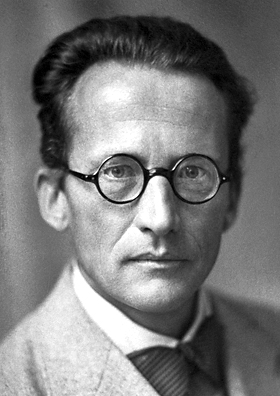
\includegraphics[width=\linewidth]{images/book3/schrodinger.jpg}
\end{minipage}\hfill
\begin{minipage}[t]{0.69\linewidth}\vspace{0pt}
{\small Erwin Schrödinger, yang pada tahun 1926 menuliskan persamaan
gelombang yang penyelesaiannya untuk atom hidrogen adalah orbital-orbital
bab ini, dan memperoleh kembali darinya tingkat-tingkat energi yang
dipostulatkan Bohr. Ia berbagi Hadiah Nobel Fisika pada tahun 1933. (Foto:
Yayasan Nobel, domain publik, Wikimedia Commons.)}
\end{minipage}
\end{omfigure}

\section{Bagian radial}

Peluang menemukan elektron di antara bola berjari-jari $r$ dan $r +
dr$ adalah $|\psi|^2$ yang diintegrasikan pada kulit bervolume
$4\pi r^2\,dr$; untuk orbital apa pun, setelah sudut-sudutnya
diintegrasikan, peluang itu adalah $r^2R^2\,dr$.

\begin{definition}[Distribusi radial]\label{def:b2:atomic-orbitals:radial-distribution}
Yang disebut \emph{fungsi distribusi radial}\index{fungsi distribusi radial}
sebuah orbital adalah $P(r) = r^2R_{nl}(r)^2$: $P(r)\,dr$ adalah peluang
elektron berada di antara $r$ dan $r + dr$ dari inti. Yang disebut
\emph{jari-jari paling mungkin}\index{jari-jari paling mungkin} adalah
nilai $r$ pada maksimum terbesarnya.
\end{definition}

\begin{proposition}[Normalisasi 1s]\label{prop:b2:atomic-orbitals:normalised}
$\int_0^\infty P_{1s}(r)\,dr = 1$.
\end{proposition}

\begin{proof}
Dengan $Z = 1$ dan $r$ dalam satuan $a_0$, $P_{1s} = 4r^2\mathrm e^{-2r}$.
Dengan integrasi parsial dua kali,
$\int_0^\infty r^2\mathrm e^{-2r}\,dr = \frac22\int_0^\infty r\,\mathrm e^{-2r}\,dr =
\frac12\int_0^\infty\mathrm e^{-2r}\,dr = \frac14$, dan $4 \times \frac14 = 1$.
\end{proof}

\begin{proposition}[Jari-jari paling mungkin]\label{prop:b2:atomic-orbitals:most-probable}
Untuk orbital 1s, \omterm{def:b2:atomic-orbitals:radial-distribution}{jari-jari paling mungkin} adalah $a_0/Z$. Untuk orbital
dengan $l =
n - 1$ (1s, 2p, 3d, \dots), jari-jari itu adalah $n^2a_0/Z$.
\end{proposition}

\begin{proof}
Untuk $l = n - 1$, \omterm{def:b2:atomic-orbitals:radial-angular}{bagian radial} tidak mempunyai simpul:
$R \propto \rho^{n-1}\mathrm e^{-\rho/n}$, sehingga
$P \propto \rho^{2n}\mathrm e^{-2\rho/n}$ dan $d\ln P/d\rho = 2n/\rho - 2/n$,
yang nol untuk $\rho = n^2$, yaitu $r = n^2a_0/Z$. Dengan $n = 1$,
$r = a_0/Z$.
\end{proof}

\begin{proposition}[Jari-jari rata-rata 1s]\label{prop:b2:atomic-orbitals:mean-radius}
Jarak rata-rata elektron 1s dari inti adalah $\langle r\rangle = 3a_0/(2Z)$,
lebih besar daripada \omterm{def:b2:atomic-orbitals:radial-distribution}{jari-jari paling mungkinnya}.
\end{proposition}

\begin{proof}
Dengan $Z = 1$: $\langle r\rangle = \int_0^\infty r\,P(r)\,dr = 4\int_0^\infty r^3\mathrm e^{-2r}
\,dr = 4 \times 3!/2^4 = 3/2$. Distribusinya mempunyai ekor panjang pada $r$
besar, yang menarik rata-ratanya melampaui maksimumnya.
\end{proof}

\begin{definition}[Simpul]\label{def:b2:atomic-orbitals:node}
Yang disebut \emph{permukaan simpul}\index{permukaan simpul} sebuah orbital
adalah permukaan tempat \omterm{def:b2:atomic-orbitals:wavefunction}{fungsi gelombang} bernilai nol dan berganti tanda.
Permukaan itu disebut \emph{simpul radial}\index{simpul radial} (sebuah
bola) jika \omterm{def:b2:atomic-orbitals:radial-angular}{bagian radialnya} lenyap, dan \emph{simpul sudut}\index{simpul sudut}
(sebuah bidang atau kerucut yang melalui inti) jika \omterm{def:b2:atomic-orbitals:radial-angular}{bagian sudutnya} yang
lenyap.
\end{definition}

\begin{proposition}[Menghitung simpul]\label{prop:b2:atomic-orbitals:nodes}
Orbital $(n, l)$ mempunyai $n - l - 1$ \omterm{def:b2:atomic-orbitals:node}{simpul radial} dan $l$ \omterm{def:b2:atomic-orbitals:node}{simpul sudut},
seluruhnya $n - 1$.
\end{proposition}

\begin{proof}
Pada fungsi-fungsi di \cref{thm:b2:atomic-orbitals:hydrogen}: $R_{2s}$ lenyap
pada $\rho = 2$, $R_{3s}$ pada kedua akar $2\rho^2 - 18\rho + 27$ ($\rho = 1.90$
dan $7.10$), $R_{3p}$ pada $\rho = 6$; $R_{1s}$, $R_{2p}$, $R_{3d}$ tidak lenyap.
\omterm{def:b2:atomic-orbitals:radial-angular}{Bagian sudut} orbital p lenyap pada satu bidang ($z = 0$ untuk $p_z$),
\omterm{def:b2:atomic-orbitals:radial-angular}{bagian sudut} orbital d pada dua bidang atau, untuk $d_{z^2}$, pada sebuah
kerucut. Kasus umumnya diterima tanpa bukti.
\end{proof}

\begin{omfigure}
\begin{tikzpicture}
\begin{axis}[width=0.55\linewidth, height=6cm, xmin=0, xmax=24, ymin=0, ymax=0.58,
  axis x line=bottom, axis y line=left, xlabel={$r/a_0$}, ylabel={$P(r)$},
  tick label style={font=\small}, label style={font=\small}, title={\small distribusi radial, $Z = 1$}]
\addplot[omThm, thick] table[x=r, y=s1] {figdata/out/bachelor-2-atomic-orbitals-a.dat};
\addplot[omDef, thick] table[x=r, y=s2] {figdata/out/bachelor-2-atomic-orbitals-a.dat};
\addplot[omDef, thick, dashed] table[x=r, y=p2] {figdata/out/bachelor-2-atomic-orbitals-a.dat};
\addplot[omProp, thick] table[x=r, y=s3] {figdata/out/bachelor-2-atomic-orbitals-a.dat};
\addplot[omProp, thick, dashed] table[x=r, y=p3] {figdata/out/bachelor-2-atomic-orbitals-a.dat};
\addplot[omProp, thick, dotted] table[x=r, y=d3] {figdata/out/bachelor-2-atomic-orbitals-a.dat};
\node[font=\scriptsize, omThm, anchor=west] at (axis cs:1.4,0.53) {1s};
\node[font=\scriptsize, omDef, anchor=south] at (axis cs:4.0,0.215) {2p};
\node[font=\scriptsize, omDef, anchor=south west] at (axis cs:6.4,0.17) {2s};
\node[font=\scriptsize, omProp, anchor=south] at (axis cs:10.5,0.12) {3d};
\node[font=\scriptsize, omProp, anchor=west] at (axis cs:17,0.085) {3s, 3p};
\end{axis}
\end{tikzpicture}\hfill
\begin{tikzpicture}
\begin{axis}[width=0.42\linewidth, height=6cm, xmin=0, xmax=20, ymin=-0.12, ymax=0.75,
  axis x line=middle, axis y line=left, xlabel={$r/a_0$}, ylabel={$R$},
  tick label style={font=\small}, label style={font=\small}, title={\small bagian radial}]
\addplot[omDef, thick] table[x=r, y=R2s] {figdata/out/bachelor-2-atomic-orbitals-b.dat};
\addplot[omProp, thick] table[x=r, y=R3s] {figdata/out/bachelor-2-atomic-orbitals-b.dat};
\node[font=\scriptsize, omDef, anchor=west] at (axis cs:0.4,0.62) {$R_{2s}$};
\node[font=\scriptsize, omProp, anchor=west] at (axis cs:0.6,0.30) {$R_{3s}$};
\node[font=\scriptsize, anchor=south west] at (axis cs:3,0.15) {simpul};
\draw[thin, ->] (axis cs:3,0.15) -- (axis cs:2.05,0.01);
\end{axis}
\end{tikzpicture}

{\small Kiri: distribusi radial $P(r) = r^2R^2$ orbital-orbital hidrogen
sampai $n = 3$; makin besar $n$, makin jauh elektronnya, dan orbital-orbital
s mempunyai maksimum dalam yang kecil (penetrasi). Kanan: $R_{2s}$ dan
$R_{3s}$ berganti tanda pada simpul-simpul radialnya ($r = 2a_0$; $1.90a_0$
dan $7.10a_0$).}
\end{omfigure}

\begin{omfigure}
\begin{tikzpicture}
\begin{axis}[scale only axis, width=0.32\linewidth, height=0.32\linewidth,
  xmin=-6, xmax=6, ymin=-6, ymax=6, axis lines=none, title={\small 1s}]
\addplot[only marks, mark=*, mark size=0.25pt, omDef] table[x=x, y=y] {figdata/out/bachelor-2-atomic-orbitals-c-1s.dat};
\end{axis}
\end{tikzpicture}\hspace{0.12\linewidth}%
\begin{tikzpicture}
\begin{axis}[scale only axis, width=0.32\linewidth, height=0.32\linewidth,
  xmin=-14, xmax=14, ymin=-14, ymax=14, axis lines=none, title={\small 2s}]
\addplot[only marks, mark=*, mark size=0.25pt, omDef] table[x=x, y=y] {figdata/out/bachelor-2-atomic-orbitals-c-2s.dat};
\draw[densely dashed, omThm] (axis cs:0,0) circle[radius=2];
\end{axis}
\end{tikzpicture}

{\small Gambar kerapatan titik orbital 1s dan 2s hidrogen pada sebuah bidang
yang melalui inti: kerapatan titik mengikuti $|\psi|^2$ (pencuplikan
deterministik). Awan 2s mempunyai cincin kosong, yaitu \omterm{def:b2:atomic-orbitals:node}{simpul radial} pada
$2a_0$ (putus-putus); bingkainya selebar 12 dan 28 $a_0$.}
\end{omfigure}

\section{Bagian sudut}

\omterm{def:b2:atomic-orbitals:radial-angular}{Bagian sudut} menetapkan bentuk. Orbital s berbentuk bola; orbital p
mempunyai dua cuping dengan tanda berlawanan di sepanjang sumbunya, yang
dipisahkan oleh bidang simpul; orbital d mempunyai empat cuping dengan
tanda berselang-seling (atau, untuk $d_{z^2}$, dua cuping dan sebuah
cincin). Tanda sebuah cuping sendiri tidak mempunyai makna fisis ---
$\psi$ dan $-\psi$ memerikan keadaan yang sama --- tetapi tanda relatif dua
orbital menentukan, pada bab berikutnya, apakah keduanya bergabung
membentuk ikatan.

\begin{omfigure}
\begin{tikzpicture}[font=\small]
  \pic at (0,0) {oms={1}};
  \node[below] at (0,-0.75) {s};
  \pic at (2.0,0) {omp={1}{0}};
  \draw[->, black!55, thin] (1.0,0) -- (3.0,0) node[right, font=\tiny] {$x$};
  \node[below] at (2.0,-0.75) {$\mathrm p_x$};
  \pic at (4.2,0) {omp={1}{90}};
  \draw[->, black!55, thin] (4.2,-0.95) -- (4.2,0.95) node[above, font=\tiny] {$z$};
  \node[below] at (4.75,-0.75) {$\mathrm p_z$};
  \pic at (6.6,0) {omdxy}; \node[below] at (6.6,-1.0) {$\mathrm d_{xy}$};
  \pic at (9.0,0) {omdx2y2}; \node[below] at (9.0,-1.0) {$\mathrm d_{x^2-y^2}$};
  \pic at (11.4,0) {omdz2}; \node[below] at (11.4,-1.0) {$\mathrm d_{z^2}$};
\end{tikzpicture}

{\small Orbital-orbital atom real, skematis: cuping-cuping menunjukkan
daerah tempat $|\psi|$ besar, diwarnai menurut tanda $\psi$ (biru positif,
oranye negatif). Orbital $\mathrm d_{xz}$ dan $\mathrm d_{yz}$ mempunyai
bentuk $\mathrm d_{xy}$ pada bidang-bidang yang ditunjukkan namanya.}
\end{omfigure}

\begin{method}[Membuat sketsa orbital dari bilangan kuantumnya]\label{met:b2:atomic-orbitals:draw-orbital}
\begin{enumerate}
  \item Dari $l$, bentuknya: s (bola), p (dua cuping), d (empat cuping, atau
        dua cuping dan sebuah cincin untuk $d_{z^2}$); dari indeksnya,
        orientasinya.
  \item Hitunglah $l$ \omterm{def:b2:atomic-orbitals:node}{simpul sudut} (bidang yang melalui inti) dan berilah
        cuping-cuping yang bersebelahan tanda yang berlawanan.
  \item Hitunglah $n - l - 1$ \omterm{def:b2:atomic-orbitals:node}{simpul radial}: kulit-kulit dalam bertanda
        berlawanan di dalam cuping utama (biasanya tidak digambar dalam
        sketsa).
  \item Skalakan dengan $n^2a_0/Z$: makin tinggi $n$, makin besar
        orbitalnya; makin besar $Z$, makin kecil.
\end{enumerate}
\end{method}

\section{Atom berelektron banyak}

Dalam atom dengan beberapa elektron, setiap elektron merasakan inti yang
ditapis oleh elektron-elektron lain. Orbital-orbitalnya mempertahankan
bentuk orbital hidrogen, dengan muatan efektif $Z^*$ menggantikan $Z$, dan
energi sebuah subkulit kini bergantung pada $l$ dan juga pada $n$: elektron
s, yang distribusi radialnya mempunyai maksimum dalam dekat inti, kurang
ditapis daripada elektron p dari kulit yang sama, dan elektron p kurang
ditapis daripada elektron d.

\begin{definition}[Aturan Slater]\label{def:b2:atomic-orbitals:slater}
Yang disebut \emph{aturan Slater}\index{aturan Slater} adalah aturan yang
memperkirakan muatan inti efektif $Z^* = Z - \sigma$ yang dirasakan sebuah
elektron. Elektron-elektron dikelompokkan sebagai
(1s) (2s, 2p) (3s, 3p) (3d) (4s, 4p) (4d) (4f) (5s, 5p) \dots; tetapan
penapisan $\sigma$ sebuah elektron adalah jumlah sumbangan elektron-elektron
lainnya: 0.35 untuk setiap elektron lain dalam kelompok yang sama (0.30 di
dalam 1s); untuk elektron s atau p, 0.85 untuk setiap elektron kulit
$n - 1$ dan 1.00 untuk setiap elektron kulit yang lebih dalam; untuk
elektron d atau f, 1.00 untuk setiap elektron kelompok di bawah kelompoknya
sendiri. Kelompok di atasnya tidak menyumbang apa pun.
\end{definition}

\begin{omfigure}
\small
\renewcommand{\arraystretch}{1.2}
\begin{tabular}{l|ccccc}
elektron yang ditinjau & kelompok sama & kulit $n - 1$ & kulit lebih dalam & kelompok di atas \\ \hline
1s & 0.30 & --- & --- & 0 \\
$n$s, $n$p & 0.35 & 0.85 & 1.00 & 0 \\
$n$d, $n$f & 0.35 & 1.00 & 1.00 & 0 \\
\end{tabular}

\smallskip
{\small Tetapan penapisan Slater, per elektron penapis. Bilangan kuantum
utama efektifnya adalah $n^* = 1, 2, 3, 3.7, 4.0, 4.2$ untuk $n = 1$ sampai
6.}
\end{omfigure}

\begin{method}[Menghitung muatan efektif]\label{met:b2:atomic-orbitals:slater}
\begin{enumerate}
  \item Tuliskan konfigurasinya dalam kelompok-kelompok Slater, menurut
        urutan $n$, dengan s dan p bersama-sama serta d dan f tersendiri.
  \item Pilihlah elektronnya; tambahkan 0.35 untuk setiap elektron lain
        dalam kelompoknya.
  \item Tambahkan 0.85 (elektron s atau p) atau 1.00 (d atau f) per elektron
        kulit tepat di bawahnya, dan 1.00 per elektron yang lebih dalam.
  \item $Z^* = Z - \sigma$.
\end{enumerate}
\end{method}

\begin{definition}[Energi dan jari-jari orbital]\label{def:b2:atomic-orbitals:orbital-energy}
Dalam model Slater, \emph{energi orbital}\index{energi orbital} sebuah
elektron dengan muatan efektif $Z^*$ dan bilangan kuantum utama efektif
$n^*$ adalah $\varepsilon = -E_RZ^{*2}/n^{*2}$, dan \emph{jari-jari
orbitalnya}\index{jari-jari orbital} adalah $n^{*2}a_0/Z^*$, yaitu
\omterm{def:b2:atomic-orbitals:radial-distribution}{jari-jari paling mungkin} orbital mirip hidrogen bermuatan $Z^*$.
\end{definition}

\begin{proposition}[Energi Slater]\label{prop:b2:atomic-orbitals:slater-energy}
Energi sekelompok $k$ elektron dengan muatan efektif $Z^*$ kira-kira
$k\varepsilon = -kE_RZ^{*2}/n^{*2}$, dan energi elektronik total atom itu
adalah jumlahnya atas semua kelompoknya.
\end{proposition}

\admitted

\begin{example}[Besi: 4s atau 3d lebih dahulu?]\label{ex:b2:atomic-orbitals:iron}
Besi adalah $[\ce{Ar}]\,3\mathrm d^6\,4\mathrm s^2$. Elektron 4s: $\sigma = 0.35 + 14
\times 0.85 + 10 \times 1.00 = 22.25$, $Z^* = 3.75$, $\varepsilon = -13.6 \times
3.75^2/3.7^2 = \qty{-14.0}{eV}$. Elektron 3d: $\sigma = 5 \times 0.35 + 18 \times 1.00 =
19.75$, $Z^* = 6.25$, $\varepsilon = -13.6 \times 6.25^2/9 = \qty{-59}{eV}$.
Elektron-elektron 3d jauh lebih kuat terikat: walaupun 4s diisi lebih
dahulu dalam urutan pengisian, elektron 4s-lah yang pergi ketika besi
diionisasi, dan ion besi(II) adalah $[\ce{Ar}]\,3\mathrm d^6$.
\end{example}

\section{Memakai energi dan ukuran orbital}

\begin{proposition}[Energi ionisasi dari energi Slater]\label{prop:b2:atomic-orbitals:ionisation}
Dalam model Slater, energi ionisasi pertama sebuah atom adalah selisih
antara energi total ion dan energi total atom, yang dihitung kelompok demi
kelompok dengan muatan efektif masing-masing.
\end{proposition}

\begin{proof}
Energi ionisasi adalah $E(\text{ion}) - E(\text{atom})$; menurut
\cref{prop:b2:atomic-orbitals:slater-energy}, keduanya merupakan jumlah
energi kelompok, dan hanya kelompok yang kehilangan elektron yang berubah
(kelompok-kelompok dalam tidak ditapis oleh elektron-elektron luar).
\end{proof}

\begin{example}[Karbon]\label{ex:b2:atomic-orbitals:carbon}
Karbon, (2s, 2p)$^4$: $Z^* = 6 - 2 \times 0.85 - 3 \times 0.35 = 3.25$; energi
kelompoknya $4 \times (-13.6 \times 3.25^2/4) = \qty{-143.6}{eV}$. Ion
\ce{C+}, (2s, 2p)$^3$: $Z^* =
3.60$, $3 \times (-13.6 \times 3.60^2/4) = \qty{-132.2}{eV}$. Energi ionisasinya \qty{11.5}{eV}, dibandingkan dengan
\qty{11.26}{eV} yang terukur.
% ledger: ie:C, const:RyhcEV
\end{example}

\begin{omfigure}
\begin{tikzpicture}
\begin{axis}[width=0.47\linewidth, height=5.4cm, xmin=0.5, xmax=8.5, ymin=0, ymax=6.5,
  axis x line=bottom, axis y line=left, xtick={1,2,3,4,5,6,7,8},
  xticklabels={Li,Be,B,C,N,O,F,Ne}, tick label style={font=\small},
  label style={font=\small}, title={\small periode 2}]
\addplot[omThm, thick, mark=*, mark size=1.3pt] table[x=k, y=zs] {figdata/out/bachelor-2-atomic-orbitals-d-period.dat};
\addplot[omDef, thick, mark=square*, mark size=1.3pt] table[x=k, y=r] {figdata/out/bachelor-2-atomic-orbitals-d-period.dat};
\node[font=\scriptsize, omThm, anchor=south east] at (axis cs:7.8,5.3) {$Z^*$};
\node[font=\scriptsize, omDef, anchor=south west] at (axis cs:1.2,3.1) {jari-jari ($a_0$)};
\end{axis}
\end{tikzpicture}\hfill
\begin{tikzpicture}
\begin{axis}[width=0.47\linewidth, height=5.4cm, xmin=1.5, xmax=6.5, ymin=0, ymax=9,
  axis x line=bottom, axis y line=left, xtick={2,3,4,5,6},
  xticklabels={Li,Na,K,Rb,Cs}, tick label style={font=\small},
  label style={font=\small}, title={\small golongan 1}]
\addplot[omThm, thick, mark=*, mark size=1.3pt] table[x=n, y=zs] {figdata/out/bachelor-2-atomic-orbitals-d-group.dat};
\addplot[omDef, thick, mark=square*, mark size=1.3pt] table[x=n, y=r] {figdata/out/bachelor-2-atomic-orbitals-d-group.dat};
\node[font=\scriptsize, omThm, anchor=north] at (axis cs:4,2.0) {$Z^*$};
\node[font=\scriptsize, omDef, anchor=west] at (axis cs:2.1,5.4) {jari-jari ($a_0$)};
\end{axis}
\end{tikzpicture}

{\small Muatan efektif Slater elektron valensi dan \omterm{def:b2:atomic-orbitals:orbital-energy}{jari-jari orbital}
$n^{*2}a_0/Z^*$. Sepanjang periode 2, $Z^*$ bertambah 0.65 per unsur dan
atom-atomnya menyusut; menuruni golongan 1, $Z^*$ tetap 1.30 lalu 2.20
sementara $n^*$ bertambah, dan atom-atomnya membesar.}
\end{omfigure}

Model ini mereproduksi kecenderungan-kecenderungan dari jilid Tahun 1.
Sepanjang periode, setiap proton tambahan hanya ditapis sebesar 0.35 oleh
elektron yang ditambahkan bersamanya: $Z^*$ naik, orbital terluar menyusut
dan mengikat lebih kuat. Menuruni golongan, $Z^*$ hampir tidak berubah
sementara kulit terluar bergerak keluar: atom-atom membesar dan energi
ionisasinya turun. Natrium, dengan $Z^* = 2.20$ untuk elektron 3s-nya,
mempunyai \omterm{def:b2:atomic-orbitals:orbital-energy}{jari-jari orbital} $9/2.2 = 4.1a_0$; klor, dengan $Z^* = 6.10$
untuk elektron 3p, $9/6.1 = 1.5a_0$.

\section{Latihan}

\begin{exercise}[$\star$]\label{exo:b2:atomic-orbitals:1}
Berikan bilangan kuantum $n$ dan $l$, jumlah \omterm{def:b2:atomic-orbitals:node}{simpul radial}, dan jumlah
\omterm{def:b2:atomic-orbitals:node}{simpul sudut} orbital 3p dan orbital 4d.
\end{exercise}

\begin{exercise}[$\star$]\label{exo:b2:atomic-orbitals:2}
Tunjukkan dari $R_{2p}$ bahwa \omterm{def:b2:atomic-orbitals:radial-distribution}{jari-jari paling mungkin} elektron 2p hidrogen
adalah $4a_0$, lalu nyatakan dalam pikometer.
\end{exercise}

\begin{exercise}[$\star$]\label{exo:b2:atomic-orbitals:3}
Hitunglah peluang menemukan elektron 1s hidrogen lebih dekat ke inti
daripada $a_0$.
\end{exercise}

\begin{exercise}[$\star$]\label{exo:b2:atomic-orbitals:4}
Sketsalah orbital $3\mathrm d_{xy}$: cuping, tanda, bidang simpul. Berapa
\omterm{def:b2:atomic-orbitals:node}{simpul radial} yang dimilikinya?
\end{exercise}

\begin{exercise}[$\star\star$]\label{exo:b2:atomic-orbitals:5}
Hitunglah muatan efektif Slater untuk elektron 2p oksigen dan \omterm{def:b2:atomic-orbitals:orbital-energy}{jari-jari
orbital} yang diberikannya.
\end{exercise}

\begin{exercise}[$\star\star$]\label{exo:b2:atomic-orbitals:6}
Dengan contoh besi, jelaskan mengapa konfigurasi \ce{Fe^3+} adalah
$[\ce{Ar}]\,3\mathrm d^5$ dan bukan $[\ce{Ar}]\,3\mathrm d^3 4\mathrm s^2$.
\end{exercise}

\begin{exercise}[$\star\star$]\label{exo:b2:atomic-orbitals:7}
Perkirakan dengan \omterm{def:b2:atomic-orbitals:slater}{aturan Slater} energi ionisasi pertama litium dan
natrium, lalu bandingkan dengan nilai terukur 5.39 dan \qty{5.14}{eV}.
Berilah komentar.
\end{exercise}

\begin{exercise}[$\star\star$]\label{exo:b2:atomic-orbitals:8}
Hitunglah $Z^*$ dan \omterm{def:b2:atomic-orbitals:orbital-energy}{jari-jari orbital} elektron terluar natrium dan klor,
lalu jelaskan mengapa atom natrium lebih besar.
\end{exercise}

\begin{exercise}[$\star\star$]\label{exo:b2:atomic-orbitals:9}
Tunjukkan bahwa orbital 1s dan 2s hidrogen ortogonal,
$\int\psi_{1s}\psi_{2s}\,dV = 0$.
\end{exercise}

\begin{exercise}[$\star\star\star$]\label{exo:b2:atomic-orbitals:10}
Tuliskan $R_{2p} = N\rho\,\mathrm e^{-\rho/2}$ dan tentukan tetapan $N$ yang
menormalisasikannya ($Z = 1$, $r$ dalam satuan $a_0$).
\end{exercise}

\begin{exercise}[$\star\star\star$]\label{exo:b2:atomic-orbitals:11}
Bandingkan jari-jari rata-rata dan \omterm{def:b2:atomic-orbitals:radial-distribution}{jari-jari paling mungkin} elektron 1s,
lalu jelaskan dari bentuk $P(r)$ mengapa keduanya berbeda.
\end{exercise}

\begin{exercise}[$\star\star\star$]\label{exo:b2:atomic-orbitals:12}
Tentukan \omterm{def:b2:atomic-orbitals:node}{permukaan simpul} orbital $\mathrm p_z$ dan tunjukkan bahwa
$\psi_{2p_z}$ berganti tanda saat melintasinya. Berapa \omterm{def:b2:atomic-orbitals:wavefunction}{kepadatan peluang}
pada permukaan itu?
\end{exercise}

\section{Soal: Di Manakah Elektron Itu?}

\begin{problem}[{Soal akhir pekan --- orbital 1s hidrogen dan
jari-jarinya, peluang menemukan elektron di luar jarak tertentu, simpul
dan maksimum 2s dan 2p, serta perkiraan Slater untuk energi ionisasi
karbon, nitrogen, dan oksigen}]
\label{pb:b2:atomic-orbitals:1}
Data: $a_0 = \qty{52.9}{pm}$; $E_R = \qty{13.6}{eV}$; energi ionisasi
pertama terukur (\unit{eV}): C 11.26, N 14.53, O 13.62. $\psi_{1s} = \pi^{-1/2}a_0^{-3/2}\,
\mathrm e^{-r/a_0}$.
% ledger: const:a0, const:RyhcEV, ie:C, ie:N, ie:O

\medskip
\noindent\textbf{Bagian I --- Orbital 1s.}
\begin{enumerate}
  \item Periksalah bahwa $\psi_{1s}$ ternormalisasi, dengan
        $dV = 4\pi r^2\,dr$.
  \item Tuliskan \omterm{def:b2:atomic-orbitals:radial-distribution}{fungsi distribusi radial} $P(r)$.
  \item Tentukan \omterm{def:b2:atomic-orbitals:radial-distribution}{jari-jari paling mungkin}.
  \item Hitunglah jari-jari rata-rata.
  \item Mengapa rata-ratanya lebih besar daripada \omterm{def:b2:atomic-orbitals:radial-distribution}{jari-jari paling mungkin}?
  \item \omterm{def:b2:atomic-orbitals:wavefunction}{Kepadatan peluang} paling besar di inti, tetapi $P(0) = 0$.
        Jelaskan.
  \item Berikan \omterm{def:b2:atomic-orbitals:radial-distribution}{jari-jari paling mungkin} dalam pikometer.
\end{enumerate}

\medskip
\noindent\textbf{Bagian II --- Di luar sebuah jari-jari.}
\begin{enumerate}[resume]
  \item Tunjukkan bahwa peluang menemukan elektron lebih jauh daripada
        $r_0 =
        xa_0$ adalah $\mathrm e^{-2x}(1 + 2x + 2x^2)$.
  \item Hitunglah peluang itu untuk $r_0 = a_0$.
  \item Hitunglah peluang itu untuk $r_0 = 2a_0$.
  \item Tentukan dengan coba-coba jari-jari bola yang memuat elektron
        dengan peluang 0.90.
  \item Dalam arti apa atom tidak mempunyai tepi, dan dalam arti apa atom
        mempunyai ukuran?
\end{enumerate}

\medskip
\noindent\textbf{Bagian III --- 2s dan 2p.}
\begin{enumerate}[resume]
  \item Berikan simpul-simpul 2s dan 2p (jumlah, jenis, posisi).
  \item Di mana $R_{2s}$ berganti tanda?
  \item Tentukan \omterm{def:b2:atomic-orbitals:radial-distribution}{jari-jari paling mungkin} 2p.
  \item Tentukan kedua maksimum $P_{2s} \propto r^2(2 - r)^2\mathrm e^{-r}$
        ($r$ dalam satuan $a_0$).
  \item Di antara 2s dan 2p, manakah yang kepadatan elektronnya lebih dekat
        ke inti? Apa akibatnya dalam atom berelektron banyak?
  \item Bagaimana jari-jari ini berubah untuk ion mirip hidrogen \ce{C^5+}?
\end{enumerate}

\medskip
\noindent\textbf{Bagian IV --- Karbon, nitrogen, oksigen.}
\begin{enumerate}[resume]
  \item Hitunglah $Z^*$ Slater elektron 2p dalam C, N, dan O.
  \item Hitunglah energi-energi orbital yang bersesuaian.
  \item Perkirakan energi ionisasi pertama karbon sebagai selisih energi
        kelompok.
  \item Hal yang sama untuk nitrogen.
  \item Hal yang sama untuk oksigen, lalu bandingkan ketiganya dengan nilai
        terukur.
  \item Ciri manakah dari nilai-nilai terukur yang luput dari model ini, dan
        mengapa?
  \item Nyatakan peluang menemukan elektron 1s hidrogen lebih jauh daripada
        $2a_0$.
\end{enumerate}
\end{problem}
